\section{Experiments}
\label{sec:experiments}

% In this section, we conduct comprehensive evaluation of \EHGRAG on four datasets. Specifically, we first compare the \EHGRAG with state-of-the-art GraphRAG methods in terms of generation accuracy. Then we test how cost-efficient and time-efficient is \EHGRAG relative to existing lightweight approaches. Finally, we conduct the ablation study to verify the contribution of each component in \EHGRAG and give the parameter sensitivity analysis to guide the parameter setting for practical usage.
% In this section, we conduct a comprehensive evaluation of EHyperGRAG. Specifically, our goal is to answer the following research questions: \textbf{Q1:} How does EHyperGRAG perform compared to state-of-the-art GraphRAG methods in terms of generation accuracy? \textbf{Q2:} How cost-efficient and time-efficient is EHyperGRAG relative to existing approaches? \textbf{Q3:} What is the contribution of structural and semantic hyperedges to the overall performance?

\subsection{Experimental Setup}

\paragraph{Datasets and Baselines.}
Following prior work~\cite{jimenez2024hipporag, zhuang2025linearrag}, we evaluate our method on four datasets including three multi-hop reasoning benchmarks: \textbf{HotpotQA} \cite{yang2018hotpotqa}, \textbf{2WikiMultiHop} \cite{xanh2020_2wikimultihop}, \textbf{MuSiQue} \cite{trivedi2022musique} and one domain-specific dataset \textbf{Medical} from GraphRAG-Bench~\cite{xiang2025use}. Detailed dataset statistics are provided in Appendix~\ref{app:datasets}. We compare \EHGRAG against two groups of baselines: (1) direct zero-shot LLM inference, including LLaMA3-8B, LLaMA3-13B~\cite{dubey2024llama3}, Qwen3-8B~\cite{yang2025qwen3}, GPT-3.5-trubo, GPT-4o-mini~\cite{openai2023gpt4} and (2) retrieval-augmented-generation methods, including vanilla RAG, KGP~\cite{wang2024knowledge}, G-retriever~\cite{he2024g}, GraphRAG~\cite{edge2024local}, RAPTOR ~\cite{sarthi2024raptor}, E$^2$GraphRAG~\cite{zhao20252graphrag}, LightRAG~\cite{guo2024lightrag}, HippoRAG~\cite{jimenez2024hipporag}, GFM-RAG~\cite{luo2025gfm}, HippoRAG2~\cite{gutiérrez2025hipporag2} and LinearRAG~\cite{zhuang2025linearrag}.

\paragraph{Evaluation Metric.}
To validate the effectiveness, we adapt two widely used metrics following existing work \cite{zhuang2025linearrag,wang2025archrag}: 1. \textbf{SubEM} utilizes whether the ground truth answer is included in the response to determine the correctness for each question. 2. \textbf{LLM-Acc} uses the LLM to assess the correctness of each response. For the Medical dataset, we only evaluate the LLM-Acc metric because the ground truth answers contain multiple statements, which makes SubEM cannot validate the effectiveness.

\paragraph{Implementation Details.}
For a fair comparison, we utilize \textbf{all-mpnet-base-v2} \cite{song2020mpnet} as the embedding model and GPT-4o-mini~\cite{openai2023gpt4} as the generator and evaluator for all methods. For the parameter $k$ in the top-$k$ retrieval, we set $k=5$ for all methods. Further details regarding machine configuration and hyperparameters are listed in Appendix~\ref{app:config}.


\subsection{Generation Performance}

\begin{table*}[ht]
\centering
\renewcommand{\arraystretch}{0.9}
\begin{tabular}{c c c c c c c c}
\toprule
\multirow{2}{*}{\textbf{Method}} & \multicolumn{2}{c}{\textbf{HotpotQA}} & \multicolumn{2}{c}{\textbf{2WikiMultiHop}} & \multicolumn{2}{c}{\textbf{MuSiQue}} & \multicolumn{1}{c}{\textbf{Medical}} \\
\cmidrule(lr){2-3} \cmidrule(lr){4-5} \cmidrule(lr){6-7} \cmidrule(lr){8-8}
& SubEM & LLM-Acc & SubEM & LLM-Acc & SubEM & LLM-Acc & LLM-Acc \\
\midrule
\multicolumn{8}{c}{\textbf{Direct Zero-shot LLM Inference}} \\
\midrule
llama-8B & 31.10 & 27.30 & 33.60 & 16.20 & 7.40 & 8.10 & 27.31 \\
llama-13B & 24.20 & 16.80 & 21.90 & 10.50 & 3.30 & 4.40 & 28.86 \\
Qwen3-8B & 25.10 & 34.70 & 29.80 & 27.10 & 6.50 & 19.80 & 58.39\\
%deepseek-r1-7B  & 25.10 & 34.70 & 29.80 & 27.10 & - & - & 58.39 \\
GPT-3.5-turbo & 33.40 & 43.20 & 28.70 & 31.00 & 10.30 & 21.90 & 45.60 \\
GPT-4o-mini & 38.90 & 40.20 & 36.30 & 31.40 & 13.60 & 15.80 & 42.10 \\
\midrule
% \multicolumn{8}{c}{\textbf{Vanilla Retrieval-Augmented-Generation}} \\
% \midrule
% Retrieval (Top-1) & 46.30 & 49.10 & 36.60 & 31.70 & 17.80 & 21.10 & 48.01 \\
% Retrieval (Top-3) & 53.00 & 56.00 & 44.90 & 39.70 & 25.10 & 27.50 & 59.07 \\
% Retrieval (Top-5) & 55.70 & 58.60 & 48.60 & 43.00 & 26.10 & 29.60 & 61.68 \\
% \midrule
\multicolumn{8}{c}{\textbf{Retrieval-Augmented-Generation Methods}} \\
\midrule
Vanilla RAG & 55.70 & 58.60 & 48.60 & 43.00 & 26.10 & 29.60 & 61.68 \\
KGP & 61.50 & 60.90 & 31.60 & 30.00 & 25.60 & 30.10 & 54.22 \\
G-retriever & 42.20 & 40.60 & 46.60 & 27.10 & 14.40 & 15.50 & 50.36 \\
GraphRAG & 58.60 & 59.80 & 49.40 & 41.60 & 24.30 & 28.70 & 48.50 \\
RAPTOR & 55.90 & 58.30 & 50.10 & 42.10 & 23.30 & 27.40 & 55.75 \\
E$^2$GraphRAG & 61.00 & 63.90 & 54.30 & 38.10 & 23.80 & 26.20 & 58.00 \\
LightRAG & 60.30 & 59.50 & 55.20 & 39.00 & 27.40 & 28.60 & 54.36 \\
HippoRAG & 57.00 & 59.30 & 66.10 & 59.90 & 29.30 & 24.10 & 55.04 \\
GFM-RAG & 62.70 & 65.60 & 66.80 & 59.60 & 29.90 & 34.60 & 56.07 \\
HippoRAG2 & 62.90 & 64.30 & 62.70 & 55.00 & 31.00 & 35.00 & 60.77 \\
LinearRAG & \underline{64.30} & \underline{66.50} & \underline{70.20} & \underline{63.70} & \underline{33.90} & \underline{37.00} & \underline{63.72} \\
\midrule
\textbf{\EHGRAG} & \textbf{65.70} & \textbf{69.30} & \textbf{73.40} & \textbf{70.60} & \textbf{34.30} & \textbf{38.40} & \textbf{65.32} \\
\bottomrule
\end{tabular}
 % End \resizebox
 \vspace{-1mm}
\caption{Result (\%) of baselines and \EHGRAG on four benchmark datasets in terms of SubEM metric and LLM Evaluation Accuracy. The best result for each dataset is highlighted in \textbf{bold}, while the second result is indicated with an \underline{underline}.}
\vspace{-2mm}
\label{tab:results}
\end{table*}

Table~\ref{tab:results} presents the results across four datasets. We observe that \EHGRAG consistently outperforms all baselines. Graph-based RAG methods generally surpass zero-shot baselines and vanilla RAG, confirming the necessity of graph construction for multi-hop reasoning. Among graph-based RAG approaches, \EHGRAG achieves superior performance. Notably, on the \textbf{2WikiMultiHop} dataset, our method achieves a substantial gain of $3.2\%$ in SubEM and $6.9\%$ in LLM-Acc over LinearRAG, which is the state-of-the-art graph-based RAG method. This dataset frequently involves reasoning chains requiring entity aliasing (e.g., linking monarch of UK to the Queen). While LinearRAG relies on structural co-occurrence within sentences, \EHGRAG utilizes semantic hyperedges and diffusion to bridge disjoint but semantically related entities, thereby enabling more robust multi-hop retrieval. Similar gains are observed on HotpotQA ($+1.4\%$ SubEM and $+2.8\%$ LLM-Acc), indicating that incorporating latent semantic correlations improves robustness without introducing significant noise.

Furthermore, on the \textbf{Medical} dataset, we observe that several LLM-heavy graph-based methods are inferior to Vanilla RAG. This phenomenon suggests that in specialized and long-context domains, relying on low-parameter LLMs for explicit graph extraction may introduce structural noise or extraction errors that degrade retrieval quality. Conversely, \EHGRAG outperforms the strongest baseline by $1.6\%$, validating the effectiveness of our proposed semantic hypergraph construction. By leveraging implicit semantic distributions rather than relying solely on rigid, LLM-extracted edges, our method maintains robustness even facing the complex domain-specific corpus.

\subsection{Ablation Study}
To understand the impact of different hyperedge types, we conduct an ablation study by removing specific components. The results are summarized in Table~\ref{tab:ablation}.

\begin{table}[ht]
\centering
\resizebox{\columnwidth}{!}{%
\begin{tabular}{l c c}
\toprule
\textbf{Variant} & \textbf{2WikiMultiHop} & \textbf{HotpotQA}\\
\midrule
\textbf{\EHGRAG (Full)} & \textbf{70.60} & \textbf{69.30} \\
w/o \textit{Sem}-Diffusion & 67.30($\downarrow 3.3\%$) & 68.50($\downarrow 0.8\%$) \\
w/o Filtering & 68.20($\downarrow 2.4\%$) & 67.90($\downarrow 1.4\%$) \\
w/o \textit{Str}-Diffusion & 66.90($\downarrow 3.7\%$) & 66.80($\downarrow 2.5\%$) \\
w/o PPR Refine & 63.10($\downarrow 7.5\%$) & 68.50($\downarrow 0.8\%$) \\
\bottomrule
\end{tabular}
}
\vspace{-1mm}
\caption{Ablation study results (LLM-Acc). \textit{Sem} means semantic and \textit{Str} means structural.}
\label{tab:ablation}
\vspace{-3mm}
\end{table}

As shown in Table~\ref{tab:ablation}, the full \EHGRAG model consistently outperforms all variants on both datasets, though the impact of specific components varies. \textit{Str}-Diffusion proves universally critical, with its removal causing significant drops on both 2WikiMultiHop (3.7\%) and HotpotQA (2.5\%), confirming the necessity of iterative structural propagation. Interestingly, \textit{Sem}-Diffusion and PPR Refine show more pronounced effects on 2WikiMultiHop (drops of 3.3\% and 7.5\%) compared to HotpotQA (0.8\% and 0.8\%). This suggests that 2WikiMultiHop contains more semantically disjoint entities and complex global dependencies, thereby relying more heavily on latent semantic bridging and global graph consistency for robust reasoning. Finally, the w/o Filtering results demonstrate that query-gated filtering consistently benefits both datasets by reducing noise. Overall, these results prove that combining structural and semantic diffusion with noise filtering and PPR refinement is essential for robust multi-hop retrieval.

\subsection{Efficiency Analysis}

We analyze the computational efficiency of \EHGRAG compared to representative baselines on the 2WikiMultiHop and HotpotQA datasets. As shown in Figure~\ref{fig:efficiency}, we report indexing time, token consumption and overall retrieval time. \EHGRAG demonstrates superior efficiency compared to LLM-heavy baselines like GraphRAG and LightRAG. It maintains zero token consumption and completes indexing in just 267.5 seconds, which is comparable to the state-of-the-art lightweight method LinearRAG, confirming that the semantic hyperedges via BIRCH clustering adds negligible computational overhead while maintaining linear complexity.

\begin{figure*}[ht] 
    \centering

    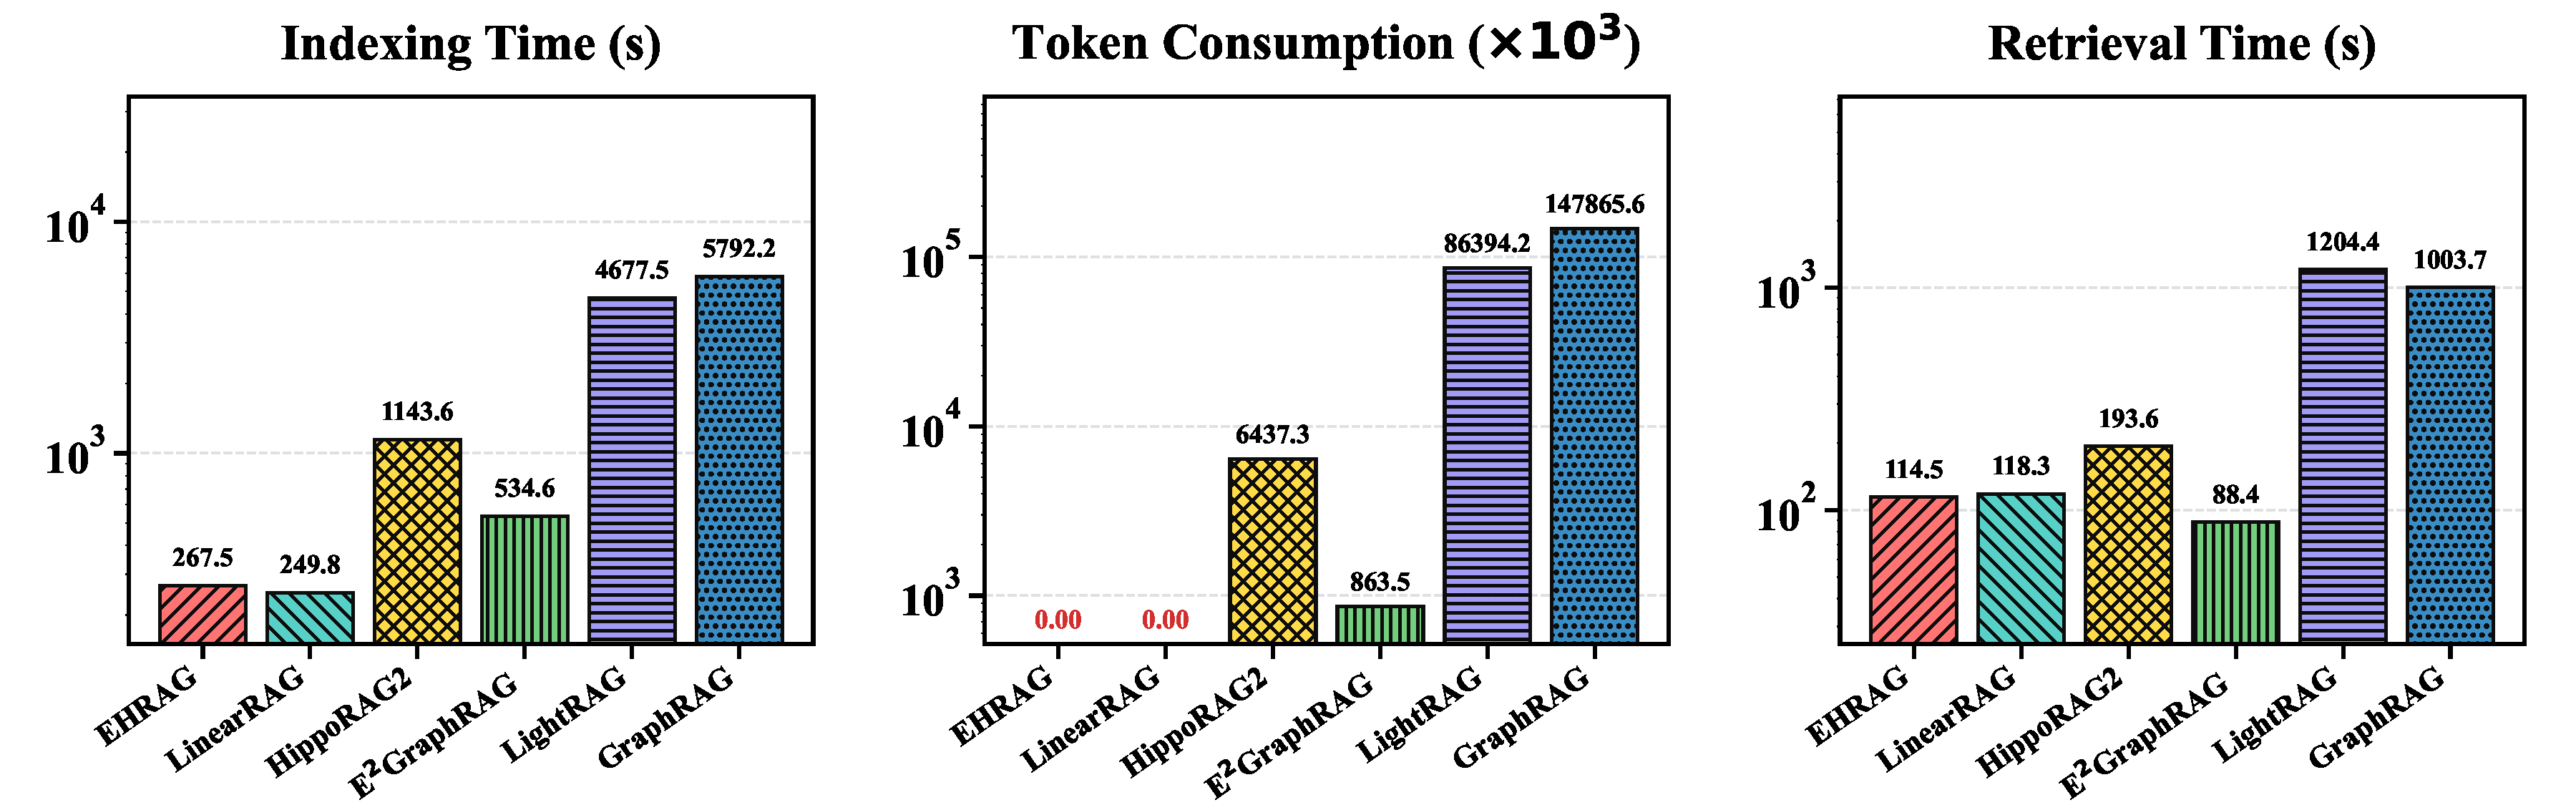
\includegraphics[width=0.9\linewidth]{figure/efficiency.pdf}
    \vspace{-1mm} 
    \caption{Efficiency comparison on 2WikiMultiHop. We report the Indexing Time, Token Consumption, and Retrieval Time for different methods. Note that the y-axis is in log scale.}
    \label{fig:efficiency}
    \vspace{-1mm} 
\end{figure*}

In terms of retrieval efficiency, \EHGRAG outperforms most baselines including HippoRAG2 and LinearRAG. While E$^2$GraphRAG exhibits slightly lower latency, it significantly lags behind state-of-the-art graph-based RAG in generation performance and needs higher indexing overhead. Consequently, \EHGRAG achieves the best balance. It possesses the most advanced multi-hop reasoning capability, and its efficiency is comparable to the most lightweight baseline.

Because the retrieval overhead is dominated by sparse matrix operations that scale linearly, the actual graph traversal takes only a fraction of a second per query. We profiled the average inference latency per query (in milliseconds) on the 2WikiMultiHop dataset using our standard hardware setup (NVIDIA RTX 4090). The detailed breakdown is presented in Table~\ref{tab:latency_breakdown}.

\begin{table}[h]
    \centering
    \begin{tabular}{lrr}
        \toprule
        \textbf{Retrieval Stage} & \textbf{Latency} & \textbf{Percent} \\
        \midrule
        1. Lightweight NER          & 21.4 ms & 18.3\% \\
        2. Entity Embedding         & 28.8 ms & 24.7\% \\
        3. Anchor Initialization    & 5.2 ms  & 4.5\%  \\
        4. Hybrid Diffusion         & 4.6 ms  & 3.9\%  \\
        5. Evidence Scoring & 21.4 ms & 18.3\% \\
        6. Topic Scoring  & 2.1 ms  & 1.8\%  \\
        7. PPR Refinement           & 33.3 ms & 28.5\% \\
        \bottomrule
    \end{tabular}
    \caption{Per-query inference latency breakdown on 2WikiMultiHop (NVIDIA RTX 4090).}
    \label{tab:latency_breakdown}
\end{table}

This detailed breakdown clearly demonstrates that our core algorithmic contributions are highly efficient. The hybrid diffusion algorithm consumes merely 4.6 milliseconds per query (only 3.9\% of the total time). Furthermore, while the overall passage scoring step takes time, our newly introduced topic-based scoring only takes 2.1 milliseconds (1.8\%). This proves that adopting a hypergraph, performing iterative diffusion, and utilizing topic scoring does not add a heavy burden to the online inference process.

Instead, the majority of the inference time is occupied by standard pipeline components. Specifically, PPR refinement (33.3 ms), entity embedding generation (28.8 ms), standard evidence scoring (21.4 ms), and lightweight NER extraction (21.4 ms) take up the bulk of the time. Since these standard steps currently dominate the retrieval process, they represent the primary ceiling for latency. Overall, this analysis confirms that the efficiency bottleneck lies in conventional pipeline components rather than in our proposed components, demonstrating that our method achieves improved retrieval quality without sacrificing inference efficiency.

\subsection{Parameter Sensitivity Analysis}
\label{sec:param_sensitivity}

\begin{figure*}[ht]
    \centering
    % 确保文件名与您 plot.py 生成的文件名一致
    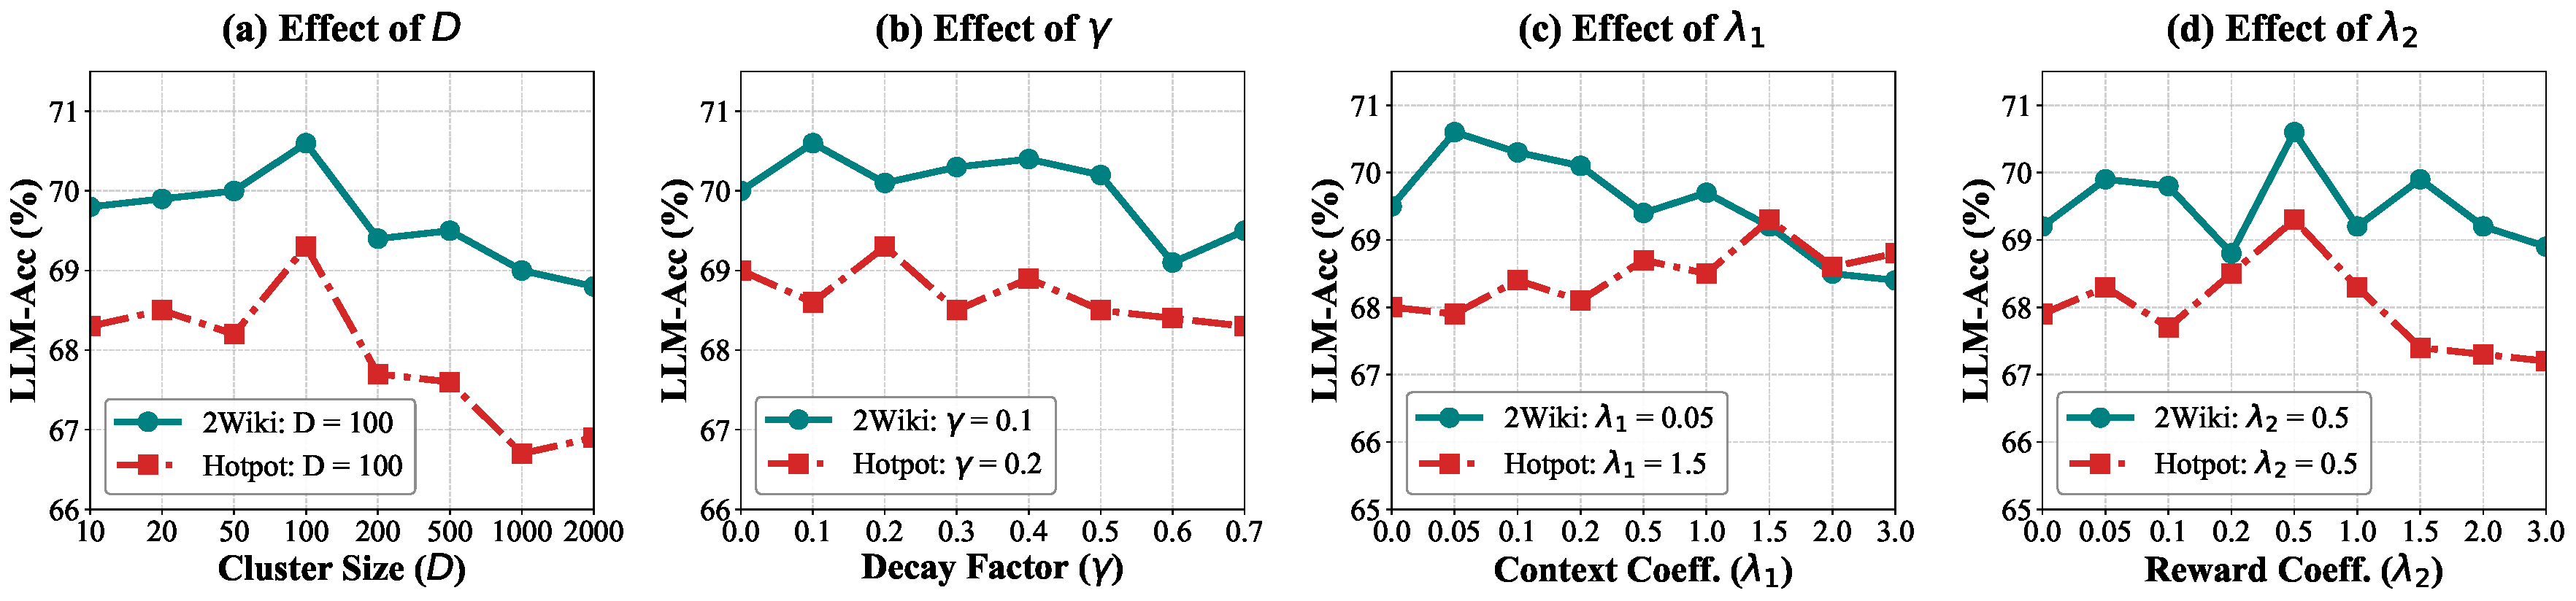
\includegraphics[width=0.95\linewidth]{figure/EHRAG_Parameter_Sensitivity.pdf}
    \vspace{-1mm}
    \caption{
    Parameter sensitivity analysis on 2WikiMultiHop (2Wiki) and HotpotQA (Hotpot) datasets. 
    }
    \label{fig:sensitivity}
    \vspace{-2mm}
\end{figure*}

To evaluate the robustness of \EHGRAG, we investigate the impact of four key hyperparameters on the 2WikiMultiHop and HotpotQA datasets including the number of nodes in a cluster $D$, the semantic propagation decay factor $\gamma$, the global context coefficient $\lambda_1$, and the semantic reward $\lambda_2$.

\textbf{Impact of Cluster Size ($D$):} The parameter $D$ controls the amount of entity within one cluster. As shown in Figure~\ref{fig:sensitivity}(a), performance initially improves as $D$ increases, peaking at $D=100$ for both datasets (70.6\% on 2WikiMultiHop and 69.3\% on HotpotQA). Setting $D$ larger than $100$ leads to a performance decline because incorporating excessive entities introduces irrelevant noise that distracts the LLM reasoning process. Thus, we recommend set $D=100$ initially for all datasets.

\textbf{Impact of Decay Factor ($\gamma$):} Figure~\ref{fig:sensitivity}(b) illustrates the effect of the semantic propagation decay factor. The model achieves optimal performance at $\gamma=0.1$ for 2WikiMultiHop and $\gamma=0.2$ for HotpotQA. This indicates that a moderate decay is necessary to maintain the focus of semantic expansion. For applying \EHGRAG on other datasets, tuning the gamma smaller than $0.5$ is recommended.

\textbf{Impact of Coefficients ($\lambda_1$ and $\lambda_2$):} Figures~\ref{fig:sensitivity}(c) and (d) analyze the balancing coefficients. For the global context coefficient $\lambda_1$, the optimal value varies significantly between datasets ($0.05$ for 2WikiMultiHop while $1.5$ for HotpotQA), suggesting that different datasets require varying degrees of global context integration. In contrast, the semantic reward coefficient $\lambda_2$ demonstrates strong stability, with both datasets achieving their peak performance at $\lambda_2=0.5$.

For other hyperparameters such as threshold $\epsilon$, sentence number $L$ and iteration number $T$, we set them based on the analysis and common values in existing studies \cite{zhuang2025linearrag,zhao20252graphrag,jimenez2024hipporag,gutiérrez2025hipporag2}. The details of all hyperparameters are listed in Appendix \ref{app:config}.

